%%%%%%%%%%%%%%%%%%%%%%%%%%%%%%%%%%%%%%%%%
% The Legrand Orange Book
% LaTeX Template
% Version 2.3 (8/8/17)
%
% This template has been downloaded from:
% http://www.LaTeXTemplates.com
%
% Original author:
% Mathias Legrand (legrand.mathias@gmail.com) with modifications by:
% Vel (vel@latextemplates.com)
%
% License:
% CC BY-NC-SA 3.0 (http://creativecommons.org/licenses/by-nc-sa/3.0/)
%
% Compiling this template:
% This template uses biber for its bibliography and makeindex for its index.
% When you first open the template, compile it from the command line with the
% commands below to make sure your LaTeX distribution is configured correctly:
%
% 1) pdflatex main
% 2) makeindex main.idx -s StyleInd.ist
% 3) biber main
% 4) pdflatex main x 2
%
% After this, when you wish to update the bibliography/index use the appropriate
% command above and make sure to compile with pdflatex several times
% afterwards to propagate your changes to the document.
%
% This template also uses a number of packages which may need to be
% updated to the newest versions for the template to compile. It is strongly
% recommended you update your LaTeX distribution if you have any
% compilation errors.
%
% Important note:
% Chapter heading images should have a 2:1 width:height ratio,
% e.g. 920px width and 460px height.
%
%%%%%%%%%%%%%%%%%%%%%%%%%%%%%%%%%%%%%%%%%

%----------------------------------------------------------------------------------------
%	PACKAGES AND OTHER DOCUMENT CONFIGURATIONS
%----------------------------------------------------------------------------------------

\documentclass[11pt,fleqn]{book} % Default font size and left-justified equations

%----------------------------------------------------------------------------------------

%%%%%%%%%%%%%%%%%%%%%%%%%%%%%%%%%%%%%%%%%
% The Legrand Orange Book
% Structural Definitions File
% Version 2.0 (9/2/15)
%
% Original author:
% Mathias Legrand (legrand.mathias@gmail.com) with modifications by:
% Vel (vel@latextemplates.com)
% 
% This file has been downloaded from:
% http://www.LaTeXTemplates.com
%
% License:
% CC BY-NC-SA 3.0 (http://creativecommons.org/licenses/by-nc-sa/3.0/)
%
%%%%%%%%%%%%%%%%%%%%%%%%%%%%%%%%%%%%%%%%%

%----------------------------------------------------------------------------------------
%	VARIOUS REQUIRED PACKAGES AND CONFIGURATIONS
%----------------------------------------------------------------------------------------

\usepackage[top=3cm,bottom=3cm,left=3cm,right=3cm,headsep=10pt,a4paper]{geometry} % Page margins

\usepackage{graphicx} % Required for including pictures
\graphicspath{{Pictures/}} % Specifies the directory where pictures are stored

\usepackage{lipsum} % Inserts dummy text

\usepackage{tikz} % Required for drawing custom shapes

\usepackage[english]{babel} % English language/hyphenation

\usepackage{enumitem} % Customize lists
\setlist{nolistsep} % Reduce spacing between bullet points and numbered lists

\usepackage{booktabs} % Required for nicer horizontal rules in tables

\usepackage{xcolor} % Required for specifying colors by name
\definecolor{ocre}{RGB}{243,102,25} % Define the orange color used for highlighting throughout the book

%----------------------------------------------------------------------------------------
%	FONTS
%----------------------------------------------------------------------------------------

\usepackage{avant} % Use the Avantgarde font for headings
%\usepackage{times} % Use the Times font for headings
\usepackage{mathptmx} % Use the Adobe Times Roman as the default text font together with math symbols from the Sym­bol, Chancery and Com­puter Modern fonts

\usepackage{microtype} % Slightly tweak font spacing for aesthetics
\usepackage[utf8]{inputenc} % Required for including letters with accents
\usepackage[T1]{fontenc} % Use 8-bit encoding that has 256 glyphs

%----------------------------------------------------------------------------------------
%	BIBLIOGRAPHY AND INDEX
%----------------------------------------------------------------------------------------

\usepackage[style=numeric,citestyle=numeric,sorting=nyt,sortcites=true,autopunct=true,babel=hyphen,hyperref=true,abbreviate=false,backref=true,backend=biber]{biblatex}
\addbibresource{bibliography.bib} % BibTeX bibliography file
\defbibheading{bibempty}{}

\usepackage{calc} % For simpler calculation - used for spacing the index letter headings correctly
\usepackage{makeidx} % Required to make an index
\makeindex % Tells LaTeX to create the files required for indexing

%----------------------------------------------------------------------------------------
%	MAIN TABLE OF CONTENTS
%----------------------------------------------------------------------------------------

\usepackage{titletoc} % Required for manipulating the table of contents

\contentsmargin{0cm} % Removes the default margin

% Part text styling
\titlecontents{part}[0cm]
{\addvspace{20pt}\centering\large\bfseries}
{}
{}
{}

% Chapter text styling
\titlecontents{chapter}[1.25cm] % Indentation
{\addvspace{12pt}\large\bfseries} % Spacing and font options for chapters
{\color{ocre!60}\contentslabel[\Large\thecontentslabel]{1.25cm}\color{ocre}} % Chapter number
{\color{ocre}}  
{\color{ocre!60}\normalsize\;\titlerule*[.5pc]{.}\;\thecontentspage} % Page number

% Section text styling
\titlecontents{section}[1.25cm] % Indentation
{\addvspace{3pt}\bfseries} % Spacing and font options for sections
{\contentslabel[\thecontentslabel]{1.25cm}} % Section number
{}
{\hfill\color{black}\thecontentspage} % Page number
[]

% Subsection text styling
\titlecontents{subsection}[1.25cm] % Indentation
{\addvspace{1pt}\small} % Spacing and font options for subsections
{\contentslabel[\thecontentslabel]{1.25cm}} % Subsection number
{}
{\ \titlerule*[.5pc]{.}\;\thecontentspage} % Page number
[]

% List of figures
\titlecontents{figure}[0em]
{\addvspace{-5pt}}
{\thecontentslabel\hspace*{1em}}
{}
{\ \titlerule*[.5pc]{.}\;\thecontentspage}
[]

% List of tables
\titlecontents{table}[0em]
{\addvspace{-5pt}}
{\thecontentslabel\hspace*{1em}}
{}
{\ \titlerule*[.5pc]{.}\;\thecontentspage}
[]

%----------------------------------------------------------------------------------------
%	MINI TABLE OF CONTENTS IN PART HEADS
%----------------------------------------------------------------------------------------

% Chapter text styling
\titlecontents{lchapter}[0em] % Indenting
{\addvspace{15pt}\large\bfseries} % Spacing and font options for chapters
{\color{ocre}\contentslabel[\Large\thecontentslabel]{1.25cm}\color{ocre}} % Chapter number
{}  
{\color{ocre}\normalsize\bfseries\;\titlerule*[.5pc]{.}\;\thecontentspage} % Page number

% Section text styling
\titlecontents{lsection}[0em] % Indenting
{\small} % Spacing and font options for sections
{\contentslabel[\thecontentslabel]{1.25cm}} % Section number
{}
{}

% Subsection text styling
\titlecontents{lsubsection}[.5em] % Indentation
{\normalfont\footnotesize} % Font settings
{}
{}
{}

%----------------------------------------------------------------------------------------
%	PAGE HEADERS
%----------------------------------------------------------------------------------------

\usepackage{fancyhdr} % Required for header and footer configuration

\pagestyle{fancy}
\renewcommand{\chaptermark}[1]{\markboth{\normalsize\bfseries\chaptername\ \thechapter.\ #1}{}} % Chapter text font settings
\renewcommand{\sectionmark}[1]{\markright{\normalsize\thesection\hspace{5pt}#1}{}} % Section text font settings
\fancyhf{} \fancyhead[LE,RO]{\normalsize\thepage} % Font setting for the page number in the header
\fancyhead[LO]{\rightmark} % Print the nearest section name on the left side of odd pages
\fancyhead[RE]{\leftmark} % Print the current chapter name on the right side of even pages
\renewcommand{\headrulewidth}{0.5pt} % Width of the rule under the header
\addtolength{\headheight}{2.5pt} % Increase the spacing around the header slightly
\renewcommand{\footrulewidth}{0pt} % Removes the rule in the footer
\fancypagestyle{plain}{\fancyhead{}\renewcommand{\headrulewidth}{0pt}} % Style for when a plain pagestyle is specified

% Removes the header from odd empty pages at the end of chapters
\makeatletter
\renewcommand{\cleardoublepage}{
\clearpage\ifodd\c@page\else
\hbox{}
\vspace*{\fill}
\thispagestyle{empty}
% \newpage
\fi}

%----------------------------------------------------------------------------------------
%	THEOREM STYLES
%----------------------------------------------------------------------------------------

\usepackage{amsmath,amsfonts,amssymb,amsthm} % For math equations, theorems, symbols, etc

\newcommand{\intoo}[2]{\mathopen{]}#1\,;#2\mathclose{[}}
\newcommand{\ud}{\mathop{\mathrm{{}d}}\mathopen{}}
\newcommand{\intff}[2]{\mathopen{[}#1\,;#2\mathclose{]}}
\newtheorem{notation}{Notation}[chapter]

% Boxed/framed environments
\newtheoremstyle{ocrenumbox}% % Theorem style name
{0pt}% Space above
{0pt}% Space below
{\normalfont}% % Body font
{}% Indent amount
{\small\bf\color{ocre}}% % Theorem head font
{\;}% Punctuation after theorem head
{0.25em}% Space after theorem head
{\small\color{ocre}\thmname{#1}\nobreakspace\thmnumber{\@ifnotempty{#1}{}\@upn{#2}}% Theorem text (e.g. Theorem 2.1)
\thmnote{\nobreakspace\the\thm@notefont\bfseries\color{black}---\nobreakspace#3.}} % Optional theorem note
\renewcommand{\qedsymbol}{$\blacksquare$}% Optional qed square

\newtheoremstyle{blacknumex}% Theorem style name
{5pt}% Space above
{5pt}% Space below
{\normalfont}% Body font
{} % Indent amount
{\small\bf}% Theorem head font
{\;}% Punctuation after theorem head
{0.25em}% Space after theorem head
{\small{\tiny\ensuremath{\blacksquare}}\nobreakspace\thmname{#1}\nobreakspace\thmnumber{\@ifnotempty{#1}{}\@upn{#2}}% Theorem text (e.g. Theorem 2.1)
\thmnote{\nobreakspace\the\thm@notefont\bfseries---\nobreakspace#3.}}% Optional theorem note

\newtheoremstyle{blacknumbox} % Theorem style name
{0pt}% Space above
{0pt}% Space below
{\normalfont}% Body font
{}% Indent amount
{\small\bf}% Theorem head font
{\;}% Punctuation after theorem head
{0.25em}% Space after theorem head
{\small\thmname{#1}\nobreakspace\thmnumber{\@ifnotempty{#1}{}\@upn{#2}}% Theorem text (e.g. Theorem 2.1)
\thmnote{\nobreakspace\the\thm@notefont\bfseries---\nobreakspace#3.}}% Optional theorem note

% Non-boxed/non-framed environments
\newtheoremstyle{ocrenum}% % Theorem style name
{5pt}% Space above
{5pt}% Space below
{\normalfont}% % Body font
{}% Indent amount
{\small\bf\color{ocre}}% % Theorem head font
{\;}% Punctuation after theorem head
{0.25em}% Space after theorem head
{\small\color{ocre}\thmname{#1}\nobreakspace\thmnumber{\@ifnotempty{#1}{}\@upn{#2}}% Theorem text (e.g. Theorem 2.1)
\thmnote{\nobreakspace\the\thm@notefont\bfseries\color{black}---\nobreakspace#3.}} % Optional theorem note
\renewcommand{\qedsymbol}{$\blacksquare$}% Optional qed square
\makeatother

% Defines the theorem text style for each type of theorem to one of the three styles above
\newcounter{dummy} 
\numberwithin{dummy}{section}
\theoremstyle{ocrenumbox}
\newtheorem{theoremeT}[dummy]{Theorem}
\newtheorem{problem}{Problem}[chapter]
\newtheorem{exerciseT}{Exercise}[chapter]
\theoremstyle{blacknumex}
\newtheorem{exampleT}{Example}[chapter]
\theoremstyle{blacknumbox}
\newtheorem{vocabulary}{Vocabulary}[chapter]
\newtheorem{definitionT}{Definition}[section]
\newtheorem{corollaryT}[dummy]{Corollary}
\theoremstyle{ocrenum}
\newtheorem{proposition}[dummy]{Proposition}

%----------------------------------------------------------------------------------------
%	DEFINITION OF COLORED BOXES
%----------------------------------------------------------------------------------------

\RequirePackage[framemethod=default]{mdframed} % Required for creating the theorem, definition, exercise and corollary boxes

% Theorem box
\newmdenv[skipabove=7pt,
skipbelow=7pt,
backgroundcolor=black!5,
linecolor=ocre,
innerleftmargin=5pt,
innerrightmargin=5pt,
innertopmargin=5pt,
leftmargin=0cm,
rightmargin=0cm,
innerbottommargin=5pt]{tBox}

% Exercise box	  
\newmdenv[skipabove=7pt,
skipbelow=7pt,
rightline=false,
leftline=true,
topline=false,
bottomline=false,
backgroundcolor=ocre!10,
linecolor=ocre,
innerleftmargin=5pt,
innerrightmargin=5pt,
innertopmargin=5pt,
innerbottommargin=5pt,
leftmargin=0cm,
rightmargin=0cm,
linewidth=4pt]{eBox}	

% Definition box
\newmdenv[skipabove=7pt,
skipbelow=7pt,
rightline=false,
leftline=true,
topline=false,
bottomline=false,
linecolor=ocre,
innerleftmargin=5pt,
innerrightmargin=5pt,
innertopmargin=0pt,
leftmargin=0cm,
rightmargin=0cm,
linewidth=4pt,
innerbottommargin=0pt]{dBox}	

% Corollary box
\newmdenv[skipabove=7pt,
skipbelow=7pt,
rightline=false,
leftline=true,
topline=false,
bottomline=false,
linecolor=gray,
backgroundcolor=black!5,
innerleftmargin=5pt,
innerrightmargin=5pt,
innertopmargin=5pt,
leftmargin=0cm,
rightmargin=0cm,
linewidth=4pt,
innerbottommargin=5pt]{cBox}

% Creates an environment for each type of theorem and assigns it a theorem text style from the "Theorem Styles" section above and a colored box from above
\newenvironment{theorem}{\begin{tBox}\begin{theoremeT}}{\end{theoremeT}\end{tBox}}
\newenvironment{exercise}{\begin{eBox}\begin{exerciseT}}{\hfill{\color{ocre}\tiny\ensuremath{\blacksquare}}\end{exerciseT}\end{eBox}}				  
\newenvironment{definition}{\begin{dBox}\begin{definitionT}}{\end{definitionT}\end{dBox}}	
\newenvironment{example}{\begin{exampleT}}{\hfill{\tiny\ensuremath{\blacksquare}}\end{exampleT}}		
\newenvironment{corollary}{\begin{cBox}\begin{corollaryT}}{\end{corollaryT}\end{cBox}}	

%----------------------------------------------------------------------------------------
%	REMARK ENVIRONMENT
%----------------------------------------------------------------------------------------

\newenvironment{remark}{\par\vspace{10pt}\small % Vertical white space above the remark and smaller font size
\begin{list}{}{
\leftmargin=35pt % Indentation on the left
\rightmargin=25pt}\item\ignorespaces % Indentation on the right
\makebox[-2.5pt]{\begin{tikzpicture}[overlay]
\node[draw=ocre!60,line width=1pt,circle,fill=ocre!25,font=\bfseries,inner sep=2pt,outer sep=0pt] at (-15pt,0pt){\textcolor{ocre}{R}};\end{tikzpicture}} % Orange R in a circle
\advance\baselineskip -1pt}{\end{list}\vskip5pt} % Tighter line spacing and white space after remark

%----------------------------------------------------------------------------------------
%	SECTION NUMBERING IN THE MARGIN
%----------------------------------------------------------------------------------------

\makeatletter
\renewcommand{\@seccntformat}[1]{\llap{\textcolor{ocre}{\csname the#1\endcsname}\hspace{1em}}}                    
\renewcommand{\section}{\@startsection{section}{1}{\z@}
{-4ex \@plus -1ex \@minus -.4ex}
{1ex \@plus.2ex }
{\normalfont\large\bfseries}}
\renewcommand{\subsection}{\@startsection {subsection}{2}{\z@}
{-3ex \@plus -0.1ex \@minus -.4ex}
{0.5ex \@plus.2ex }
{\normalfont\bfseries}}
\renewcommand{\subsubsection}{\@startsection {subsubsection}{3}{\z@}
{-2ex \@plus -0.1ex \@minus -.2ex}
{.2ex \@plus.2ex }
{\normalfont\small\bfseries}}                        
\renewcommand\paragraph{\@startsection{paragraph}{4}{\z@}
{-2ex \@plus-.2ex \@minus .2ex}
{.1ex}
{\normalfont\small\bfseries}}

%----------------------------------------------------------------------------------------
%	PART HEADINGS
%----------------------------------------------------------------------------------------

% numbered part in the table of contents
\newcommand{\@mypartnumtocformat}[2]{%
\setlength\fboxsep{0pt}%
\noindent\colorbox{ocre!20}{\strut\parbox[c][.7cm]{\ecart}{\color{ocre!70}\Large\bfseries\centering#1}}\hskip\esp\colorbox{ocre!40}{\strut\parbox[c][.7cm]{\linewidth-\ecart-\esp}{\Large\centering#2}}}%
%%%%%%%%%%%%%%%%%%%%%%%%%%%%%%%%%%
% unnumbered part in the table of contents
\newcommand{\@myparttocformat}[1]{%
\setlength\fboxsep{0pt}%
\noindent\colorbox{ocre!40}{\strut\parbox[c][.7cm]{\linewidth}{\Large\centering#1}}}%
%%%%%%%%%%%%%%%%%%%%%%%%%%%%%%%%%%
\newlength\esp
\setlength\esp{4pt}
\newlength\ecart
\setlength\ecart{1.2cm-\esp}
\newcommand{\thepartimage}{}%
\newcommand{\partimage}[1]{\renewcommand{\thepartimage}{#1}}%
\def\@part[#1]#2{%
\ifnum \c@secnumdepth >-2\relax%
\refstepcounter{part}%
\addcontentsline{toc}{part}{\texorpdfstring{\protect\@mypartnumtocformat{\thepart}{#1}}{\partname~\thepart\ ---\ #1}}
\else%
\addcontentsline{toc}{part}{\texorpdfstring{\protect\@myparttocformat{#1}}{#1}}%
\fi%
\startcontents%
\markboth{}{}%
{\thispagestyle{empty}%
\begin{tikzpicture}[remember picture,overlay]%
\node at (current page.north west){\begin{tikzpicture}[remember picture,overlay]%	
\fill[ocre!20](0cm,0cm) rectangle (\paperwidth,-\paperheight);
\node[anchor=north] at (4cm,-3.25cm){\color{ocre!40}\fontsize{220}{100}\bfseries\thepart}; 
\node[anchor=south east] at (\paperwidth-1cm,-\paperheight+1cm){\parbox[t][][t]{8.5cm}{
\printcontents{l}{0}{\setcounter{tocdepth}{1}}%
}};
\node[anchor=north east] at (\paperwidth-1.5cm,-3.25cm){\parbox[t][][t]{15cm}{\strut\raggedleft\color{white}\fontsize{30}{30}\bfseries#2}};
\end{tikzpicture}};
\end{tikzpicture}}%
\@endpart}
\def\@spart#1{%
\startcontents%
\phantomsection
{\thispagestyle{empty}%
\begin{tikzpicture}[remember picture,overlay]%
\node at (current page.north west){\begin{tikzpicture}[remember picture,overlay]%	
\fill[ocre!20](0cm,0cm) rectangle (\paperwidth,-\paperheight);
\node[anchor=north east] at (\paperwidth-1.5cm,-3.25cm){\parbox[t][][t]{15cm}{\strut\raggedleft\color{white}\fontsize{30}{30}\bfseries#1}};
\end{tikzpicture}};
\end{tikzpicture}}
\addcontentsline{toc}{part}{\texorpdfstring{%
\setlength\fboxsep{0pt}%
\noindent\protect\colorbox{ocre!40}{\strut\protect\parbox[c][.7cm]{\linewidth}{\Large\protect\centering #1\quad\mbox{}}}}{#1}}%
\@endpart}
\def\@endpart{\vfil
% \newpage
\if@twoside
\if@openright
\null
\thispagestyle{empty}%
% \newpage
\fi
\fi
\if@tempswa
\twocolumn
\fi}

%----------------------------------------------------------------------------------------
%	CHAPTER HEADINGS
%----------------------------------------------------------------------------------------

% A switch to conditionally include a picture, implemented by  Christian Hupfer
\newif\ifusechapterimage
\usechapterimagetrue
\newcommand{\thechapterimage}{}%
\newcommand{\chapterimage}[1]{\ifusechapterimage\renewcommand{\thechapterimage}{#1}\fi}%
\newcommand{\autodot}{.}
\def\@makechapterhead#1{%
{\parindent \z@ \raggedright \normalfont
\ifnum \c@secnumdepth >\m@ne
\if@mainmatter
\begin{tikzpicture}[remember picture,overlay]
\node at (current page.north west)
{\begin{tikzpicture}[remember picture,overlay]
\node[anchor=north west,inner sep=0pt] at (0,0) {\ifusechapterimage\includegraphics[width=\paperwidth]{\thechapterimage}\fi};
\draw[anchor=west] (\Gm@lmargin,-9cm) node [line width=2pt,rounded corners=15pt,draw=ocre,fill=white,fill opacity=0.5,inner sep=15pt]{\strut\makebox[22cm]{}};
\draw[anchor=west] (\Gm@lmargin+.3cm,-9cm) node {\huge\bfseries\color{black}\thechapter\autodot~#1\strut};
\end{tikzpicture}};
\end{tikzpicture}
\else
\begin{tikzpicture}[remember picture,overlay]
\node at (current page.north west)
{\begin{tikzpicture}[remember picture,overlay]
\node[anchor=north west,inner sep=0pt] at (0,0) {\ifusechapterimage\includegraphics[width=\paperwidth]{\thechapterimage}\fi};
\draw[anchor=west] (\Gm@lmargin,-9cm) node [line width=2pt,rounded corners=15pt,draw=ocre,fill=white,fill opacity=0.5,inner sep=15pt]{\strut\makebox[22cm]{}};
\draw[anchor=west] (\Gm@lmargin+.3cm,-9cm) node {\huge\bfseries\color{black}#1\strut};
\end{tikzpicture}};
\end{tikzpicture}
\fi\fi\par\vspace*{270\p@}}}

%-------------------------------------------

\def\@makeschapterhead#1{%
\begin{tikzpicture}[remember picture,overlay]
\node at (current page.north west)
{\begin{tikzpicture}[remember picture,overlay]
\node[anchor=north west,inner sep=0pt] at (0,0) {\ifusechapterimage\includegraphics[width=\paperwidth]{\thechapterimage}\fi};
\draw[anchor=west] (\Gm@lmargin,-9cm) node [line width=2pt,rounded corners=15pt,draw=ocre,fill=white,fill opacity=0.5,inner sep=15pt]{\strut\makebox[22cm]{}};
\draw[anchor=west] (\Gm@lmargin+.3cm,-9cm) node {\huge\bfseries\color{black}#1\strut};
\end{tikzpicture}};
\end{tikzpicture}
\par\vspace*{270\p@}}
\makeatother

%----------------------------------------------------------------------------------------
%	HYPERLINKS IN THE DOCUMENTS
%----------------------------------------------------------------------------------------

\usepackage{hyperref}
\hypersetup{hidelinks,backref=true,pagebackref=true,hyperindex=true,colorlinks=false,breaklinks=true,urlcolor= ocre,bookmarks=true,bookmarksopen=false,pdftitle={Title},pdfauthor={Author}}
\usepackage{bookmark}
\bookmarksetup{
open,
numbered,
addtohook={%
\ifnum\bookmarkget{level}=0 % chapter
\bookmarksetup{bold}%
\fi
\ifnum\bookmarkget{level}=-1 % part
\bookmarksetup{color=ocre,bold}%
\fi
}
}


% custom add package
\usepackage{fontspec}
\usepackage[UTF8]{ctex}
\usepackage{xeCJK}
\usepackage{verbatim}
\usepackage{lmodern}
\setmainfont{Times}
\setCJKmainfont{Songti TC}
% \setCJKmainfont{Xingkai TC} % Insert the commands.tex file which contains the majority of the structure behind the template

%\usepackage{ctexcap}
%\usepackage[heading]{ctex}
\usepackage[UTF8]{ctex}
\usepackage{verbatim}


\begin{document}

%----------------------------------------------------------------------------------------
%	TITLE PAGE
%----------------------------------------------------------------------------------------

\begingroup
\thispagestyle{empty}
\begin{tikzpicture}[remember picture,overlay]
\node[inner sep=0pt] (background) at (current page.center) {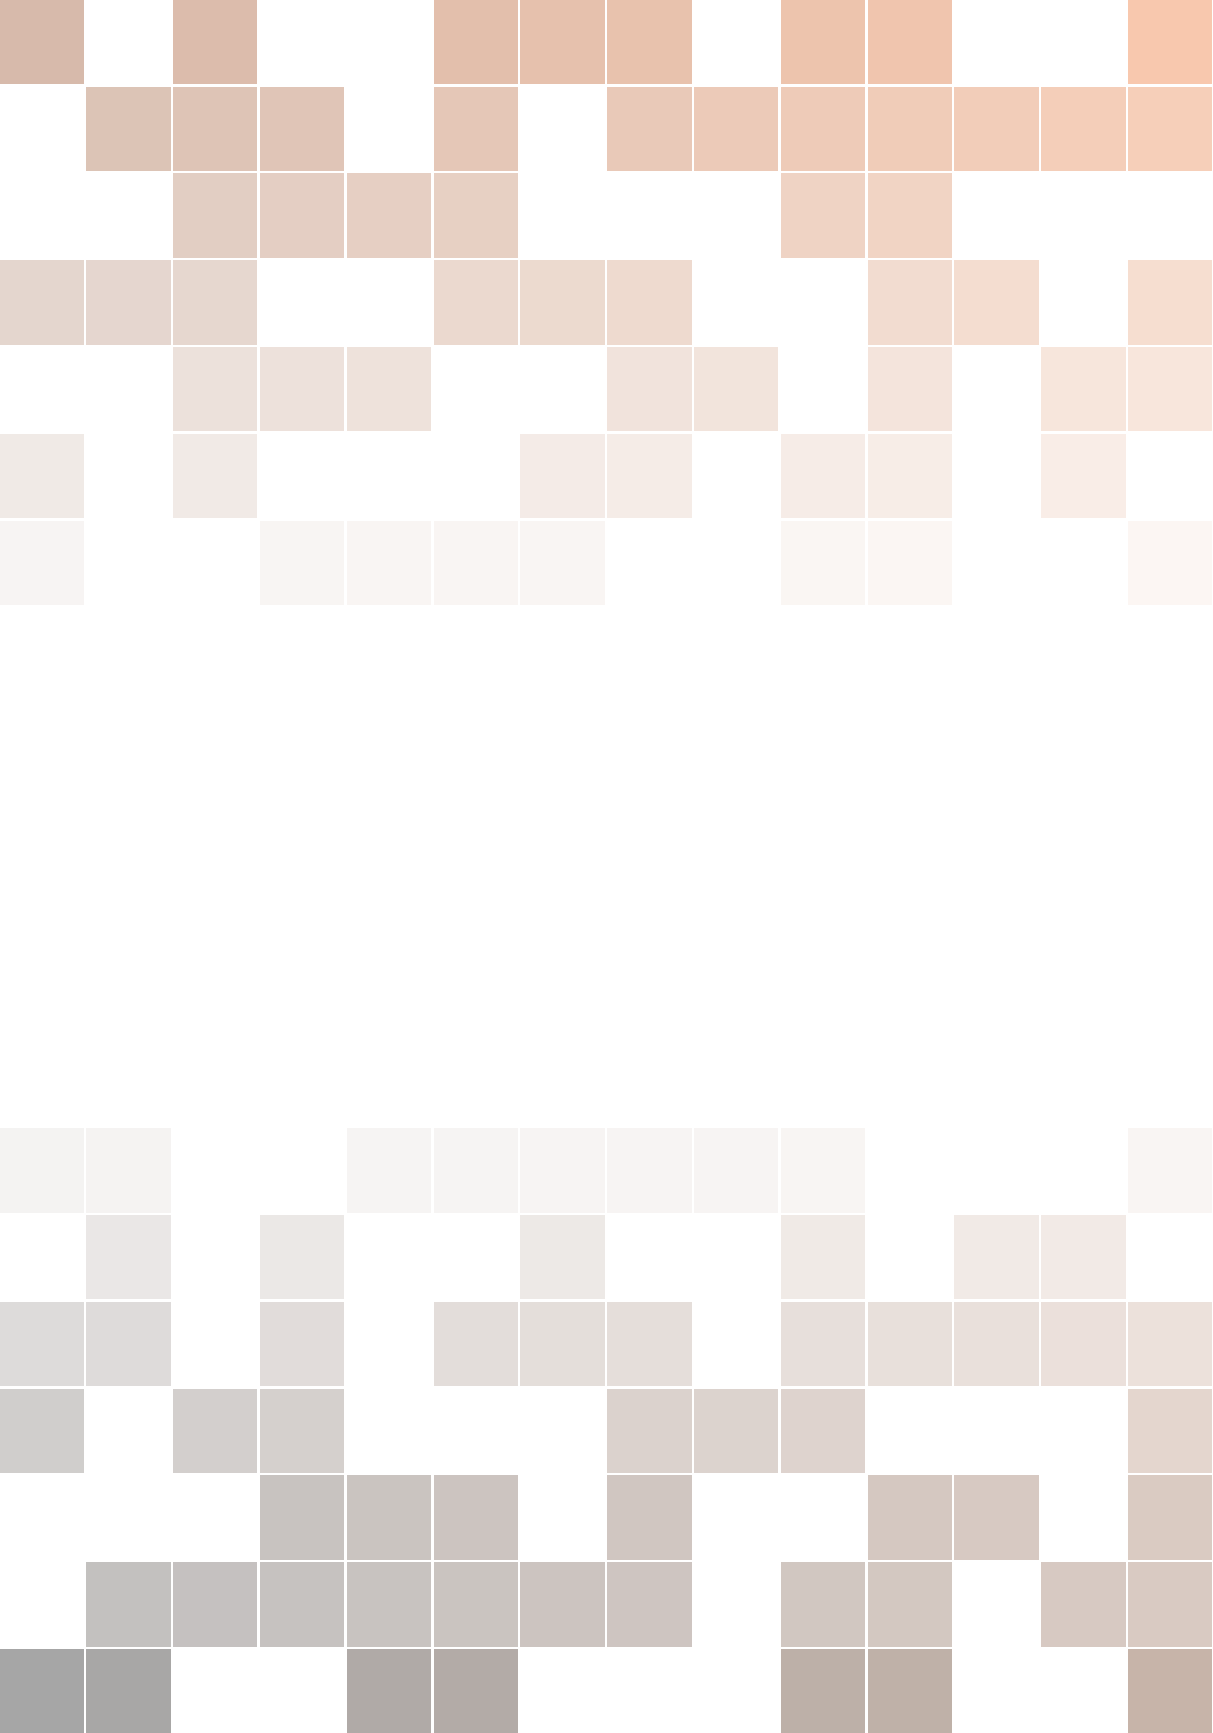
\includegraphics[width=\paperwidth]{background}};
\draw (current page.center) node [fill=ocre!30!white,fill opacity=0.6,text opacity=1,inner sep=1cm]
{
\Huge\centering\bfseries\sffamily\parbox[c][][t]{\paperwidth}
 {\centering
 古文精選\\[30pt] % Book title
% 文心雕龍\\[20pt] % Subtitle
 {\huge 采采流水}
 }
}; % Author name
\end{tikzpicture}
\vfill
\endgroup

%----------------------------------------------------------------------------------------
%	COPYRIGHT PAGE
%----------------------------------------------------------------------------------------

\newpage
~\vfill
\thispagestyle{empty}

\noindent Copyright \copyright\ 2013 John Smith\\ % Copyright notice

\noindent \textsc{Published by Publisher}\\ % Publisher

\noindent \textsc{book-website.com}\\ % URL

\noindent Licensed under the Creative Commons Attribution-NonCommercial 3.0 Unported License (the ``License''). You may not use this file except in compliance with the License. You may obtain a copy of the License at \url{http://creativecommons.org/licenses/by-nc/3.0}. Unless required by applicable law or agreed to in writing, software distributed under the License is distributed on an \textsc{``as is'' basis, without warranties or conditions of any kind}, either express or implied. See the License for the specific language governing permissions and limitations under the License.\\ % License information

\noindent \textit{First printing, March 2017} % Printing/edition date

%----------------------------------------------------------------------------------------
%	TABLE OF CONTENTS
%----------------------------------------------------------------------------------------

%\usechapterimagefalse % If you don't want to include a chapter image, use this to toggle images off - it can be enabled later with \usechapterimagetrue

\chapterimage{chapter_head_1.pdf} % Table of contents heading image

\pagestyle{empty} % No headers

\tableofcontents % Print the table of contents itself

\cleardoublepage % Forces the first chapter to start on an odd page so it's on the right

\pagestyle{fancy} % Print headers again

%----------------------------------------------------------------------------------------
%	PART
%----------------------------------------------------------------------------------------

\part{Part One}

%----------------------------------------------------------------------------------------
%	CHAPTER 1
%----------------------------------------------------------------------------------------

\chapterimage{chapter_head_2.pdf} % Chapter heading image

%\chapter{Text Chapter}
\chapter{此情可待}

\section{ 伶官传序}

呜呼!盛衰之理,虽曰天命,岂非人事哉!原庄宗之所以得天下,与其所以失之者,可以知之矣。

世言晋王之将终也,以三矢赐庄宗而告之曰:“梁,吾仇也;燕王,吾所立,契丹与吾约为兄弟,而皆背晋以归梁。此三者,吾遗恨也。与尔三矢,尔其无忘乃父之志!”庄宗受而藏之于庙。其后用兵,则遣从事以一少牢告庙,请其矢,盛以锦囊,负而前驱,及凯旋而纳之。

方其系燕父子以组,函梁君臣之首,入于太庙,还矢先王,而告以成功,其意气之盛,可谓壮哉!及仇雠已灭,天下已定,一夫夜呼,乱者四应,仓皇东出,未及见贼而士卒离散,君臣相顾,不知所归,至于誓天断发,泣下沾襟,何其衰也!岂得之难而失之易欤?抑本其成败之迹, 而皆自于人欤?《书》曰:“满招损,谦受益。” 忧劳可以兴国,逸豫可以亡身,自然之理也。

故方其盛也,举天下豪杰,莫能与之争;及其衰也,数十伶人困之,而身死国灭,为天下笑。夫祸患常积于忽微,而智勇多困于所溺,岂独伶人也哉!




\section{ 聊齋自序}
披萝带荔,三闾氏感而为骚;牛鬼蛇神,长爪郎吟而成癖。自鸣天籁,不择好音,有由然矣。松落落秋萤之火,魑魅争光;逐逐野马之尘,魍魉见笑。才非干宝,雅爱搜神;情类黄州,喜人谈鬼。闻则命笔,遂以成编。久之,四方同人又以邮筒相寄,因而物以好聚,所积益夥。甚者:人非化外,事或奇于断发之乡;睫在眼前,怪有过于飞头之国。遄飞逸兴,狂固难辞;永托旷怀,痴且不讳。展如之人,得勿向我胡卢耶?然五爷衢头,或涉滥听;而三生石上,颇悟前因。放纵之言,有未可概以人废者。松悬弧时,先大人梦一病瘠瞿昙偏袒入室,药膏如钱,圆粘乳际。寤而松生,果符墨志。且也,少羸多病,长命不犹。门庭之凄寂,则冷淡如僧;笔墨之耕耘,则萧条似钵。每搔头自念,勿亦面壁人果吾前身耶?盖有漏根因,未结人天之果;而随风荡堕,竟成藩溷之花。茫茫六道,何可谓无其理哉!独是子夜荧荧,灯昏欲蕊;萧斋瑟瑟,案冷疑冰。集腋为裘,妄续幽冥之录;浮白载笔,仅成孤愤之书。寄托如此,亦足悲矣!嗟乎!惊霜寒雀,抱树无温;吊月秋虫,偎栏自热。知我者,其在青林黑塞间乎!

\section{ 遊褒禪山記}

褒禅山亦谓之华山,唐浮图慧褒始舍于其址,而卒葬之;以故其后名之曰“褒禅”。今所谓慧空禅院者,褒之庐冢也。距其院东五里,所谓华山洞者,以其乃华山之阳名之也。距洞百余步,有碑仆道,其文漫灭,独其为文犹可识曰“花山”。今言“华”如“华实”之“华”者,盖音谬也。

其下平旷,有泉侧出,而记游者甚众,所谓前洞也。由山以上五六里,有穴窈然,入之甚寒,问其深,则其好游者不能穷也,谓之后洞。余与四人拥火以入,入之愈深,其进愈难,而其见愈奇。有怠而欲出者,曰:“不出,火且尽。”遂与之俱出。盖余所至,比好游者尚不能十一,然视其左右,来而记之者已少。盖其又深,则其至又加少矣。方是时,余之力尚足以入,火尚足以明也。既其出,则或咎其欲出者,而余亦悔其随之,而不得极夫游之乐也。

于是余有叹焉。古人之观于天地、山川、草木、虫鱼、鸟兽,往往有得,以其求思之深而无不在也。夫夷以近,则游者众;险以远,则至者少。而世之奇伟、瑰怪,非常之观,常在于险远,而人之所罕至焉,故非有志者不能至也。有志矣,不随以止也,然力不足者,亦不能至也。有志与力,而又不随以怠,至于幽暗昏惑而无物以相之,亦不能至也。然力足以至焉,于人为可讥,而在己为有悔;尽吾志也而不能至者,可以无悔矣,其孰能讥之乎?此余之所得也!

余于仆碑,又以悲夫古书之不存,后世之谬其传而莫能名者,何可胜道也哉!此所以学者不可以不深思而慎取之也。

四人者:庐陵萧君圭君玉,长乐王回深父,余弟安国平父、安上纯父。

至和元年七月某日,临川王某记

\section{ 陳情表——李密}

臣密言:臣以险衅,夙遭闵凶。生孩六月,慈父见背;行年四岁,舅夺母志。祖母刘愍臣孤弱,躬亲抚养。臣少多疾病,九岁不行,零丁孤苦,至于成立。既无伯叔,终鲜兄弟,门衰祚薄,晚有儿息。外无期功强近之亲,内无应门五尺之僮,茕茕孑立,形影相吊。而刘夙婴疾病,常在床蓐,臣侍汤药,未曾废离。

逮奉圣朝,沐浴清化。前太守臣逵察臣孝廉;后刺史臣荣举臣秀才。臣以供养无主,辞不赴命。诏书特下,拜臣郎中,寻蒙国恩,除臣洗马。猥以微贱,当侍东宫,非臣陨首所能上报。臣具以表闻,辞不就职。诏书切峻,责臣逋慢;郡县逼迫,催臣上道;州司临门,急于星火。臣欲奉诏奔驰,则刘病日笃,欲苟顺私情,则告诉不许。臣之进退,实为狼狈。

伏惟圣朝以孝治天下,凡在故老,犹蒙矜育,况臣孤苦,特为尤甚。且臣少仕伪朝,历职郎署,本图宦达,不矜名节。今臣亡国贱俘,至微至陋,过蒙拔擢,宠命优渥,岂敢盘桓,有所希冀!但以刘日薄西山,气息奄奄,人命危浅,朝不虑夕。臣无祖母,无以至今日,祖母无臣,无以终余年。母孙二人,更相为命,是以区区不能废远。

臣密今年四十有四,祖母今年九十有六,是臣尽节于陛下之日长,报养刘之日短也。乌鸟私情,愿乞终养。臣之辛苦,非独蜀之人士及二州牧伯所见明知,皇天后土,实所共鉴。愿陛下矜悯愚诚,听臣微志,庶刘侥幸,保卒余年。臣生当陨首,死当结草。臣不胜犬马怖惧之情,谨拜表以闻。

\section{ 項脊軒志——归有光}

项脊轩,旧南阁子也。室仅方丈,可容一人居。百年老屋,尘泥渗漉,雨泽下注;每移案,顾视,无可置者。又北向,不能得日,日过午已昏。余稍为修葺,使不上漏。前辟四窗,垣墙周庭,以当南日,日影反照,室始洞然。又杂植兰桂竹木于庭,旧时栏楯,亦遂增胜。借书满架,偃仰啸歌,冥然兀坐,万籁有声;而庭堦寂寂,小鸟时来啄食,人至不去。三五之夜,明月半墙,桂影斑驳,风移影动,珊珊可爱。

然余居于此,多可喜,亦多可悲。先是庭中通南北为一。迨诸父异爨,内外多置小门,墙往往而是。东犬西吠,客逾庖而宴,鸡栖于厅。庭中始为篱,已为墙,凡再变矣。家有老妪,尝居于此。妪,先大母婢也,乳二世,先妣抚之甚厚。室西连于中闺,先妣尝一至。妪每谓余曰:“某所,而母立于兹。”妪又曰:“汝姊在吾怀,呱呱而泣;娘以指叩门扉曰:‘儿寒乎?欲食乎?’吾从板外相为应答。”语未毕,余泣,妪亦泣。余自束发,读书轩中,一日,大母过余曰:“吾儿,久不见若影,何竟日默默在此,大类女郎也?”比去,以手阖门,自语曰:“吾家读书久不效,儿之成,则可待乎!”顷之,持一象笏至,曰:“此吾祖太常公宣德间执此以朝,他日汝当用之!”瞻顾遗迹,如在昨日,令人长号不自禁。

轩东,故尝为厨,人往,从轩前过。余扃牖而居,久之,能以足音辨人。轩凡四遭火,得不焚,殆有神护者。

项脊生曰:“蜀清守丹穴,利甲天下,其后秦皇帝筑女怀清台;刘玄德与曹操争天下,诸葛孔明起陇中。方二人之昧昧于一隅也,世何足以知之,余区区处败屋中,方扬眉、瞬目,谓有奇景。人知之者,其谓与坎井之蛙何异?”

余既为此志,后五年,吾妻来归,时至轩中,从余问古事,或凭几学书。吾妻归宁,述诸小妹语曰:"闻姊家有阁子,且何谓阁子也?"其后六年,吾妻死,室坏不修。其后二年,余久卧病无聊,乃使人复葺南阁子,其制稍异于前。然自后余多在外,不常居。

庭有枇杷树,吾妻死之年所手植也,今已亭亭如盖矣。


\section{ 与妻书——林觉民}

意映卿卿如晤:

吾今以此书与汝永别矣!吾作此书时,尚为世中一人;汝看此书时,吾已成为阴间一鬼。吾作此书,泪珠和笔墨齐下,不能竟书而欲搁笔。又恐汝不察吾衷,谓吾忍舍汝而死,谓吾不知汝之不欲吾死也,故遂忍悲为汝言之。

吾至爱汝!即此爱汝一念,使吾勇于就死也!吾自遇汝以来,常愿天下有情人都成眷属,然遍地腥云,满街狼犬,称心快意,几家能够?司马青衫,吾不能学太上之忘情也。语云,仁者“老吾老以及人之老,幼吾幼以及人之幼”。吾充吾爱汝之心,助天下人爱其所爱,所以敢先汝而死,不顾汝也。汝体吾此心,于悲啼之余,亦以天下人为念,当亦乐牺牲吾身与汝身之福利,为天下人谋永福也。汝其勿悲。

汝忆否四五年前某夕,吾尝语曰:“与使吾先死也,无宁汝先吾而死。”汝初闻言而怒,后经吾婉解,虽不谓吾言为是,而亦无辞相答。吾之意盖谓以汝之弱,必不能禁失吾之悲,吾先死留苦与汝,吾心不忍,故宁请汝先死,吾担悲也。嗟夫,谁知吾卒先汝而死乎!

吾真不能忘汝也!回忆后街之屋,入门穿廊,过前后厅,又三四折有小厅,厅旁一室为吾与汝双栖之所。初婚三四个月,适冬之望日前后,窗外疏梅筛月影,依稀掩映,吾与汝并肩携手,低低切切,何事不语,何情不诉!及今思之,空余泪痕!又回忆六七年前,吾之逃家复归也,汝泣告我:“望今后有远行,必以告妾,妾愿随君行。”吾亦既许汝矣。前十余日回家,即欲乘便以此行之事语汝,及与汝相对,又不能启口;且以汝之有身也,更恐不胜悲,故惟日日呼酒买醉。嗟夫!当时余心之悲,盖不能以寸管形容之。

吾诚愿与汝相守以死。第以今日事势观之,天灾可以死,盗贼可以死,瓜分之日可以死,奸官污吏虐民可以死,吾辈处今日之中国,国中无地无时不可以死!到那时使吾眼睁睁看汝死,或使汝眼睁睁看我死,吾能之乎!抑汝能之乎!即可不死,而离散不相见,徒使两地眼成穿而骨化石,试问古来几曾见破镜能重圆,则较死为苦也。将奈之何?今日吾与汝幸双健;天下人人不当死而死,与不愿离而离者,不可数计;钟情如我辈者,能忍之乎?此吾所以敢率性就死不顾汝也!吾今死无余憾,国事成不成,自有同志者在。依新已五岁,转眼成人,汝其善抚之,使之肖我。汝腹中之物,吾疑其女也,女必像汝,吾心甚慰;或又是男,则亦教其以父志为志,则我死后,尚有二意洞在也,甚幸甚幸!

吾家后日当甚贫,贫无所苦,清静过日而已。

吾今与汝无言矣!吾居九泉之下,遥闻汝哭声,当哭相和也。吾平日不信有鬼,今则又望其真有。今人又言心电感应有道,吾亦望其言是实,则吾之死,吾灵尚依依旁汝也,汝不必以无侣悲!

吾生平未尝以吾所志语汝,是吾不是处。然语之,又恐汝日日为吾担忧。吾牺牲百死而不辞,而使汝担忧,的的非吾所忍。吾爱汝至,所以为汝谋者惟恐未尽。汝幸而偶我,又何不幸而生今日之中国!吾幸而得汝,又何不幸而生今日之中国,卒不忍独善其身!嗟夫!巾短情长,所未尽者尚有万千,汝可摹拟得之。吾今不能见汝矣!汝不能舍吾,其时时于梦中寻我乎!一恸!

辛亥三月念六夜四鼓,意洞手书。

家中诸母皆通文,有不解处,望请其指教。当尽吾意为幸

\section{ 祭十二郎文}

年、月、日,季父愈闻汝丧之七日,乃能衔哀致诚,使建中远具时羞之奠,告汝十二郎之灵:

呜呼!吾少孤,及长,不省所怙,惟兄嫂是依。中年,兄殁南方,吾与汝俱幼,从嫂归葬河阳。既又与汝就食江南。零丁孤苦,未尝一日相离也。吾上有三兄,皆不幸早世。承先人后者,在孙惟汝,在子惟吾。两世一身,形单影只。嫂尝抚汝指吾而言曰:“韩氏两世,惟此而已!”汝时尤小,当不复记忆。吾时虽能记忆,亦未知其言之悲也。

吾年十九,始来京城。其后四年,而归视汝。又四年,吾往河阳省坟墓,遇汝从嫂丧来葬。又二年,吾佐董丞相于汴州,汝来省吾。止一岁,请归取其孥。明年,丞相薨。吾去汴州,汝不果来。是年,吾佐戎徐州,使取汝者始行,吾又罢去,汝又不果来。吾念汝从于东,东亦客也,不可以久。图久远者,莫如西归,将成家而致汝。呜呼!孰谓汝遽去吾而殁乎!吾与汝俱少年,以为虽暂相别,终当久相与处,故舍汝而旅食京师,以求斗斛之禄。诚知其如此,虽万乘之公相,吾不以一日辍汝而就也。

去年,孟东野往。吾书与汝曰:“吾年未四十,而视茫茫,而发苍苍,而齿牙动摇。念诸父与诸兄,皆康强而早逝。如吾之衰者,其能久存乎?吾不可去,汝不肯来,恐旦暮死,而汝抱无涯之戚也!”孰谓少者殁而长者存,强者夭而病者全乎!

呜呼!其信然邪?其梦邪?其传之非其真邪?信也,吾兄之盛德而夭其嗣乎?汝之纯明而不克蒙其泽乎?少者、强者而夭殁,长者、衰者而存全乎?未可以为信也。梦也,传之非其真也,东野之书,耿兰之报,何为而在吾侧也?呜呼!其信然矣!吾兄之盛德而夭其嗣矣!汝之纯明宜业其家者,不克蒙其泽矣!所谓天者诚难测,而神者诚难明矣!所谓理者不可推,而寿者不可知矣!

虽然,吾自今年来,苍苍者或化而为白矣,动摇者或脱而落矣。毛血日益衰,志气日益微,几何不从汝而死也。死而有知,其几何离;其无知,悲不几时,而不悲者无穷期矣。

汝之子始十岁,吾之子始五岁。少而强者不可保,如此孩提者,又可冀其成立邪!呜呼哀哉!呜呼哀哉!

汝去年书云:“比得软脚病,往往而剧。”吾曰:“是疾也,江南之人,常常有之。”未始以为忧也。呜呼!其竟以此而殒其生乎?抑别有疾而至斯乎?汝之书,六月十七日也。东野云,汝殁以六月二日;耿兰之报无月日。盖东野之使者,不知问家人以月日;如耿兰之报,不知当言月日。东野与吾书,乃问使者,使者妄称以应之耳。其然乎?其不然乎?

今吾使建中祭汝,吊汝之孤与汝之乳母。彼有食,可守以待终丧,则待终丧而取以来;如不能守以终丧,则遂取以来。其余奴婢,并令守汝丧。吾力能改葬,终葬汝于先人之兆,然后惟其所愿。

呜呼!汝病吾不知时,汝殁吾不知日,生不能相养于共居,殁不能抚汝以尽哀,敛不凭其棺,窆不临其穴。吾行负神明,而使汝夭;不孝不慈,而不能与汝相养以生,相守以死。一在天之涯,一在地之角,生而影不与吾形相依,死而魂不与吾梦相接。吾实为之,其又何尤!彼苍者天,曷其有极!自今已往,吾其无意于人世矣!当求数顷之田于伊颍之上,以待馀年,教吾子与汝子,幸其成;长吾女与汝女,待其嫁,如此而已。

呜呼!言有穷而情不可终,汝其知也邪!其不知也邪!呜呼哀哉!尚飨!





\part{Part Two}

%----------------------------------------------------------------------------------------
%	CHAPTER 2
%----------------------------------------------------------------------------------------

% \chapterimage{chapter_head_1.pdf} % Chapter heading image

\chapter{ 文采飞扬}
\section{ 洛神赋}

黄初三年,余朝京师,还济洛川。古人有言,斯水之神,名曰宓妃。感宋玉对楚王神女之事,遂作斯赋,其词曰:

余从京域,言归东藩,背伊阙 ,越轘辕,经通谷,陵景山。日既西倾,车殆马烦。尔乃税驾乎蘅皋,秣驷乎芝田,容与乎阳林,流眄乎洛川。于是精移神骇,忽焉思散。俯则未察,仰以殊观。睹一丽人,于岩之畔。乃援御者而告之曰:“尔有觌于彼者乎?彼何人斯,若此之艳也!”御者对曰:“臣闻河洛之神,名曰宓妃。然则君王所见,无乃是乎?其状若何,臣愿闻之。”

余告之曰:其形也,翩若惊鸿,婉若游龙,荣曜秋菊,华茂春松。髣髴兮若轻云之蔽月,飘飖兮若流风之回雪。远而望之,皎若太阳升朝霞。迫而察之,灼若芙蕖出渌波。秾纤得衷,修短合度。肩若削成,腰如约素。延颈秀项,皓质呈露,芳泽无加,铅华弗御。云髻峨峨,修眉联娟,丹唇外朗,皓齿内鲜。明眸善睐,靥辅承权,瓌姿艳逸,仪静体闲。柔情绰态,媚于语言。奇服旷世,骨像应图。披罗衣之璀粲兮,珥瑶碧之华琚。戴金翠之首饰,缀明珠以耀躯。践远游之文履,曳雾绡之轻裾。微幽兰之芳蔼兮,步踟蹰于山隅。于是忽焉纵体,以遨以嬉。左倚采旄,右荫桂旗。攘皓腕于神浒兮,采湍濑之玄芝。

余情悦其淑美兮,心振荡而不怡。无良媒以接欢兮,托微波而通辞。愿诚素之先达兮,解玉佩以要之。嗟佳人之信修兮,羌习礼而明诗。抗琼珶以和予兮,指潜渊而为期。执眷眷之款实兮,惧斯灵之我欺。感交甫之弃言兮,怅犹豫而狐疑。收和颜而静志兮,申礼防以自持。

于是洛灵感焉,徙倚彷徨。神光离合,乍阴乍阳。竦轻躯以鹤立,若将飞而未翔。践椒涂之郁烈,步蘅薄而流芳。超长吟以永慕兮,声哀厉而弥长。 尔乃众灵杂遝,命俦啸侣。或戏清流,或翔神渚。或采明珠,或拾翠羽。从南湘之二妃,携汉滨之游女。叹匏瓜之无匹兮,咏牵牛之独处。扬轻袿之猗靡兮,翳修袖以延伫。体迅飞凫,飘忽若神。凌波微步,罗袜生尘。动无常则,若危若安。进止难期,若往若还。转眄流精,光润玉颜。含辞未吐,气若幽兰。华容婀娜,令我忘餐。

于是屏翳收风,川后静波。冯夷鸣鼓,女娲清歌。腾文鱼以警乘,鸣玉鸾以偕逝。六龙俨其齐首,载云车之容裔。鲸鲵踊而夹毂,水禽翔而为卫。于是越北沚,过南冈,纡素领,回清阳,动朱唇以徐言,陈交接之大纲。恨人神之道殊兮,怨盛年之莫当。抗罗袂以掩涕兮,泪流襟之浪浪。悼良会之永绝兮,哀一逝而异乡。无微情以效爱兮,献江南之明珰。虽潜处于太阴,长寄心于君王。忽不悟其所舍,怅神宵而蔽光。

于是背下陵高,足往神留。遗情想像,顾望怀愁。冀灵体之复形,御轻舟而上溯。浮长川而忘返,思绵绵而增慕。夜耿耿而不寐,沾繁霜而至曙。命仆夫而就驾,吾将归乎东路。揽騑辔以抗策,怅盘桓而不能去。

\section{ 滕王阁序——王勃}
豫章故郡,洪都新府。星分翼轸,地接衡庐。襟三江而带五湖,控蛮荆而引瓯越。物华天宝,龙光射牛斗之墟;人杰地灵,徐孺下陈蕃之榻。雄州雾列,俊采星驰。台隍枕夷夏之交,宾主尽东南之美。都督阎公之雅望,棨戟遥临;宇文新州之懿范,襜帷暂驻。十旬休假,胜友如云;千里逢迎,高朋满座。腾蛟起凤,孟学士之词宗;紫电青霜,王将军之武库。家君作宰,路出名区;童子何知,躬逢胜饯。

时维九月,序属三秋。潦水尽而寒潭清,烟光凝而暮山紫。俨骖騑于上路,访风景于崇阿。临帝子之长洲,得仙人之旧馆。层峦耸翠,上出重霄;飞阁流丹,下临无地。鹤汀凫渚,穷岛屿之萦回;桂殿兰宫,即冈峦之体势。

披绣闼,俯雕甍,山原旷其盈视,川泽纡其骇瞩。闾阎扑地,钟鸣鼎食之家;舸舰迷津,青雀黄龙之舳。云销雨霁,彩彻区明。落霞与孤鹜齐飞,秋水共长天一色。渔舟唱晚,响穷彭蠡之滨,雁阵惊寒,声断衡阳之浦。

遥襟甫畅,逸兴遄飞。爽籁发而清风生,纤歌凝而白云遏。睢园绿竹,气凌彭泽之樽;邺水朱华,光照临川之笔。四美具,二难并。穷睇眄于中天,极娱游于暇日。天高地迥,觉宇宙之无穷;兴尽悲来,识盈虚之有数。望长安于日下,目吴会于云间。地势极而南溟深,天柱高而北辰远。关山难越,谁悲失路之人;萍水相逢,尽是他乡之客。怀帝阍而不见,奉宣室以何年?

嗟乎!时运不齐,命途多舛。冯唐易老,李广难封。屈贾谊于长沙,非无圣主;窜梁鸿于海曲,岂乏明时?所赖君子见机,达人知命。老当益壮,宁移白首之心?穷且益坚,不坠青云之志。酌贪泉而觉爽,处涸辙以犹欢。北海虽赊,扶摇可接;东隅已逝,桑榆非晚。孟尝高洁,空余报国之情;阮籍猖狂,岂效穷途之哭!

勃,三尺微命,一介书生。无路请缨,等终军之弱冠;有怀投笔,慕宗悫之长风。舍簪笏于百龄,奉晨昏于万里。非谢家之宝树,接孟氏之芳邻。他日趋庭,叨陪鲤对;今兹捧袂,喜托龙门。杨意不逢,抚凌云而自惜;钟期既遇,奏流水以何惭?

呜乎!胜地不常,盛筵难再;兰亭已矣,梓泽丘墟。临别赠言,幸承恩于伟饯;登高作赋,是所望于群公。敢竭鄙怀,恭疏短引;一言均赋,四韵俱成。请洒潘江,各倾陆海云尔:

% \begin{verbatim}
\begin{verse}
\hspace{2.5cm}  滕王高阁临江渚,佩玉鸣鸾罢歌舞。\\
\hspace{2.5cm}  画栋朝飞南浦云,珠帘暮卷西山雨。\\
\hspace{2.5cm}  闲云潭影日悠悠,物换星移几度秋。\\
\hspace{2.5cm}  阁中帝子今何在?槛外长江空自流。\\
\end{verse}
% \end{verbatim}



\part{Part Three}

%----------------------------------------------------------------------------------------
%	CHAPTER 3
%----------------------------------------------------------------------------------------



\chapter{ 興觀群怨}

\section{百字令(投袁大琴南)——龚自珍}


深情似海,问相逢初度,是何年纪?依约而今还记取,不是前生夙世。放学花前,题诗石上,春水园亭里。逢君一笑,人间无此欢喜。


无奈苍狗看云,红羊数劫,惘惘休提起!客气渐多真气少,汩没心灵何已?千古声名,百年担负,事事违初意。心头阁住,儿时那种情味。





%----------------------------------------------------------------------------------------
%	BIBLIOGRAPHY
%----------------------------------------------------------------------------------------

\chapter*{Bibliography}
\addcontentsline{toc}{chapter}{\textcolor{ocre}{Bibliography}}

%------------------------------------------------

\section*{Articles}
\addcontentsline{toc}{section}{Articles}
\printbibliography[heading=bibempty,type=article]

%------------------------------------------------

\section*{Books}
\addcontentsline{toc}{section}{Books}
\printbibliography[heading=bibempty,type=book]

%----------------------------------------------------------------------------------------
%	INDEX
%----------------------------------------------------------------------------------------

\cleardoublepage
\phantomsection
\setlength{\columnsep}{0.75cm}
\addcontentsline{toc}{chapter}{\textcolor{ocre}{Index}}
\printindex

%----------------------------------------------------------------------------------------

\end{document}
